\chapter{User Manual}
\label{appendix-user-manual}

\begin{center}
  \begin{figure}[ht!]
    \makebox[\textwidth]{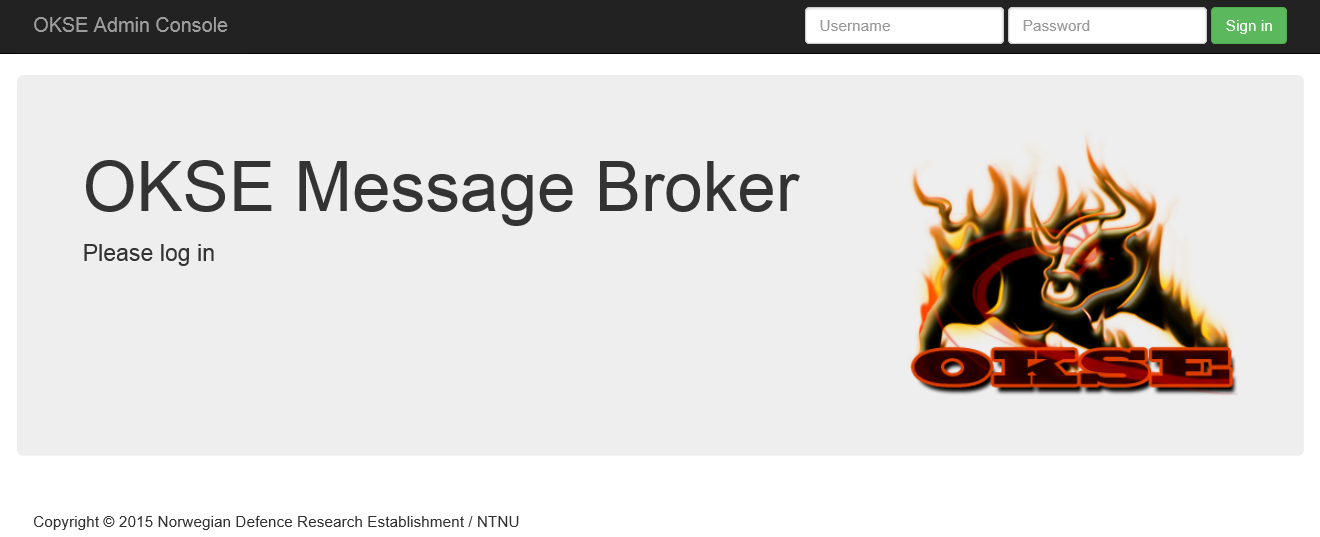
\includegraphics[width=\textwidth]{fig/oac/oac.png}}
    \caption{The OKSE Admin Console login page} 
    \label{fig:OKSE Admin Console login page}
  \end{figure}
\end{center}

\section{About}

This chapter contains instructions for installing and using the OKSE Message Broker. The intended users are primarily researchers working with collaborative networking. OKSE is open source, and licensed under the MIT license.

\section{Requirements}

OKSE Message Broker requires a Java Runtime Environment (hereby denoted as JRE) version 8 update 31 or newer, to be able to run. The broker is developed and tested exclusively with this version. The software is available for free from Oracle.com\footnote{\url{http://www.oracle.com/technetwork/java/javase/downloads/jre8-downloads-2133155.html}}.

For the JRE to function properly, it must be added to the path variable. On UNIX-based systems, like Linux or OS X, it is done by entering the following command in the terminal: \verb!export JAVA_HOME=<PATH-TO-JRE>!. On windows, open up a command line window(cmd.exe) and type in  \verb!path %path%;<PATH-TO-JRE>!.
The variable can also be accessed and modified through the "Environmental variables" tab in the advanced system settings. The system should be possible to run on all platforms with JRE installed. 

In addition to JRE, OKSE requires a network connection to be able to send and receive messages. It does not however, require Internet on the connection. 

\section{Installation}

The following sections describes how to download and run OKSE. Apart from JRE, no other additional configuration should be necessary.

\subsection{Download software}

Download the latest version of OKSE Message Broker from [URL HERE].
The file can placed in an appropriate place in the file system. For example: \verb!$HOME/okse/! on UNIX-based systems, and \verb!C:\Program Files\okse\! on Windows.

\subsection{Running the software}

On Windows, the broker can be started by double-clicking on the .jar-file. On UNIX-based systems and Windows alike, the broker is started by running the command: \\ \verb!java -jar <PATH-TO-JAR-FILE>/<JAR-FILE>.jar! from the command line or terminal.

See section \ref{sec:inital-login} for information about accessing the administration panel.

\section{Configuration}

After the initial start up of OKSE Message Broker, there is created a folder named \verb!config! in the same location as the .jar-file. This folder contains three configuration files with the default configuration:

\begin{itemize}
\setlength{\itemsep}{0cm}%
\item okse.properties
\item log4j.properties
\item topicmapping.properties
\end{itemize}

\noindent See section \ref{sec:configuration_files} for detailed information about all the possible settings.

\section{Inital login}
\label{sec:inital-login}

After launching the application, the administrator interface should be reachable from any web browser. By default, the admin console is accessible from \verb!localhost:8080!. Both the host and port can be changed in the okse.properties (see section \ref{subsec:configuration_files-okse.properties}). To log in the first time, use \verb!admin! and \verb!password! as respectively username and password. To increase the security, it is recommended that this is changed immediately after the initial login. 

\begin{itemize}
\setlength{\itemsep}{0cm}%
\item Default host and port for admin console: \verb!localhost:8080!
\item Default username and password: \verb!admin! and \verb!password!
\end{itemize}

\section{Admin Console}
The OKSE Admin Console provides information about OKSE and it's operation enviroment. It also gives access to configure OKSE. The interface have information sorted in six panes, the Main pane, the Topic pane, the Subscribers pane and the Configuration pane.

\subsection{The Main pane}
The Main pane is an overview of the broker's status, system, the operating environment, interfaces and ports the different protocol servers are bound to. It's worth mentioning that the RAM reported is RAM available in Java Virtaual Machine. It is also possible to stop and start the protocol servers from the interface section. When you stop and start the protocol servers again, the statistics are reset to zero.

\begin{center}
  \begin{figure}[ht!]
    \makebox[\textwidth]{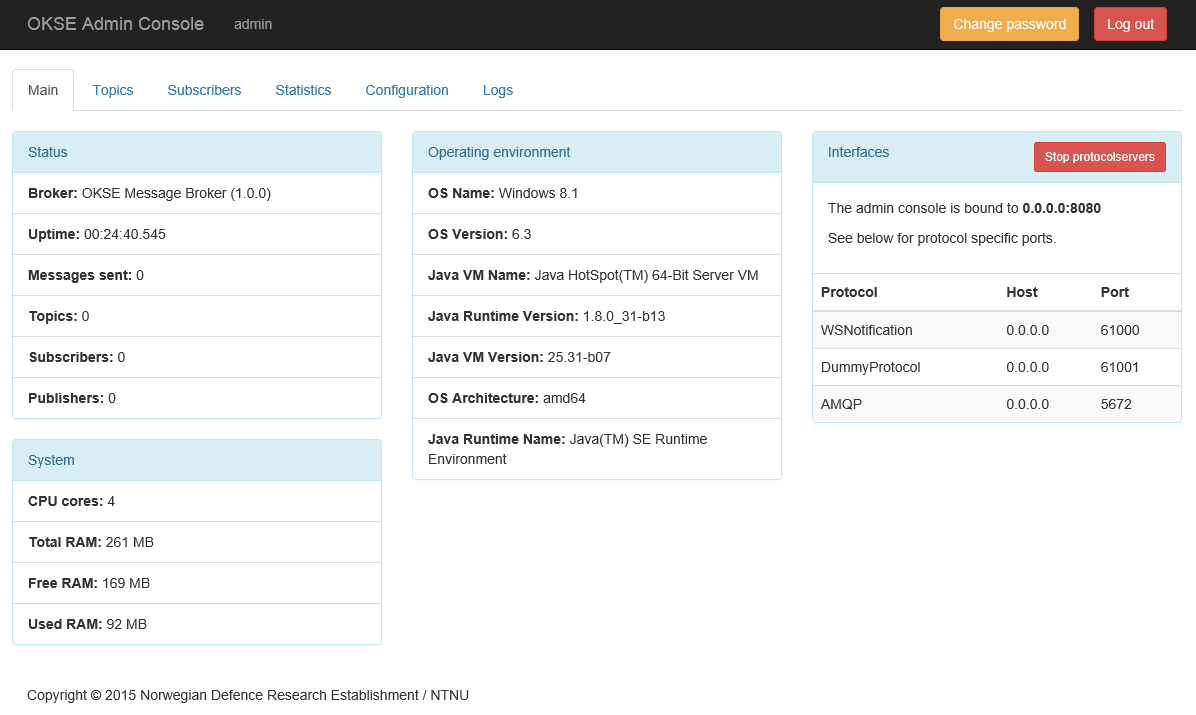
\includegraphics[width=\textwidth]{fig/oac/mainpane.png}}
    \caption{The OKSE Admin Console - Main pane} 
    \label{fig:OKSE Admin Console - Main pane}
  \end{figure}
\end{center}

\subsection{The Topics pane}
The Topics pane contains all the registered topics in OKSE. For each topic it is possible to see how many clients are subscribing to the topic (---comment about xpath not being subscribers??---). It is also possible to delete all topics or a specific topic. The 'Stop refresh'-button stops the automatic refreshing of the topic list. This can be usefull when there are many new topic are generated, and you do not want the list to update (ex: you want to search in the list)

\begin{center}
  \begin{figure}[ht!]
    \makebox[\textwidth]{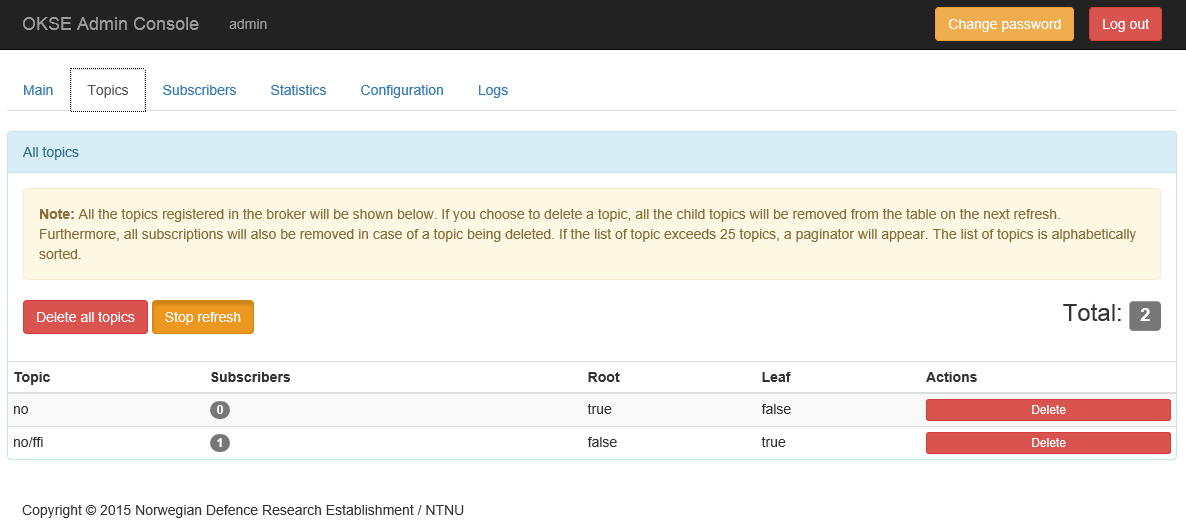
\includegraphics[width=\textwidth]{fig/oac/topicspane.png}}
    \caption{The OKSE Admin Console - Topics pane} 
    \label{fig:OKSE Admin Console - Topics pane}
  \end{figure}
\end{center}

\subsection{The Subscribers pane}
The subscribers pane shows all the subscribers (hosts). It also lists which protocol the subscriber are using, on which port, and if any filters are specified. One or all users can be deleted, denoted as unsubscribe in WSN and disconnect in AMQP. The 'Stop refresh'-button stops the automatic refreshing of the subscription list. This can be use full when there are many clients subscribing and/or unsubscribing, and you do not want the list to update (ex: you want to search in the list)

\begin{center}
  \begin{figure}[ht!]
    \makebox[\textwidth]{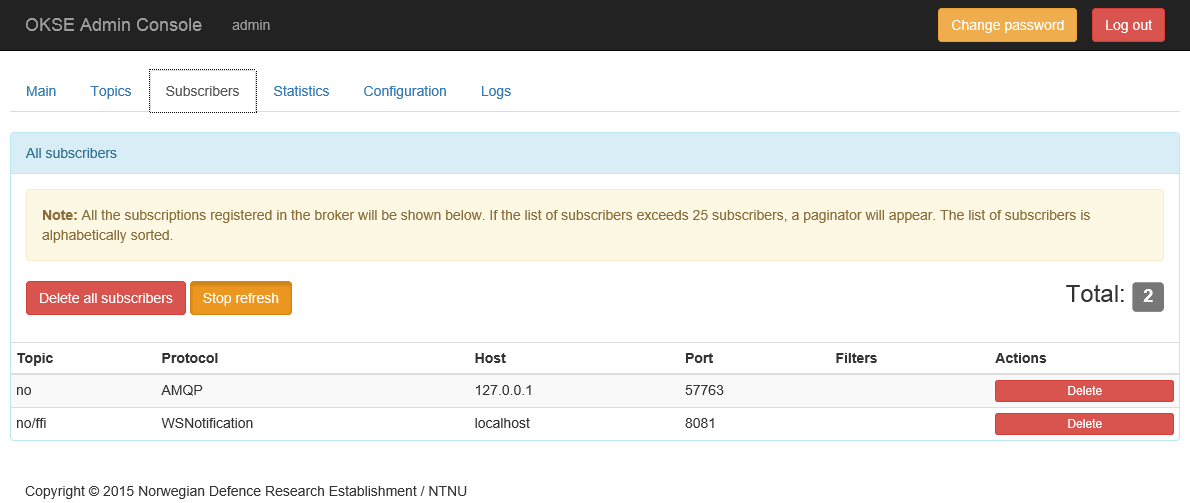
\includegraphics[width=\textwidth]{fig/oac/subscriptionspane.png}}
    \caption{The OKSE Admin Console - Subscriptions pane} 
    \label{fig:OKSE Admin Console - Subscriptions pane}
  \end{figure}
\end{center}

\subsection{The Statistics pane}
The Statistics pane prvides a list of protocol servers with statistics per protocol and total usage. "Sent" denotes the amount of messages sent on the different protocols. "Received" denotes messages received on current protocol. "Requests" are the total amount of requests on the protocol. The WSNotification protocol server "Requests" are subscribe request, message sendt to the broker, publisher registration, and trying to acccess an endpoint address. For AMQP a request are countet when the broker got a socket connection, and when a message is sendt to the broker. "Bad request" on the WSNotification protocol server can be trying to access an WSNotification endpoint. AMQP does not count "Bad requests". Errors are counted on WSNotification when OKSE try to send a message, but can not reach the subscriber. For AMQP errors are counted when some one try to connect to OKSE on AMQP's port, but the connection is not accepted. In the usage panel you get the total stats for all protocols.

\begin{center}
  \begin{figure}[ht!]
    \makebox[\textwidth]{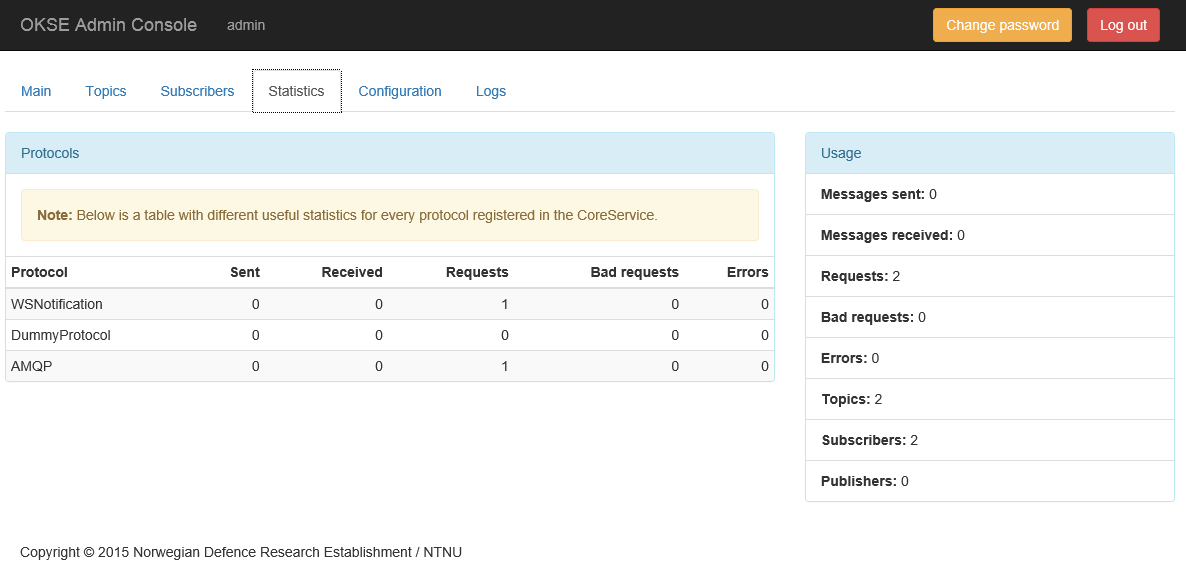
\includegraphics[width=\textwidth]{fig/oac/statisticspane.png}}
    \caption{The OKSE Admin Console - Statistics pane} 
    \label{fig:OKSE Admin Console - Statistics pane}
  \end{figure}
\end{center}

\subsection{The Configuration pane}
The Configuration pane has three sections; options, topic mapping and relays. In the option section you can change the auto update interval for refreshing the web page. The "Use AMQP queues instead of pub/sub topics" changes the queue semantic.

In the topic mapping section one can manually map from one topic to another one. The mapping is an simplex action. If a mapping is made between topic A and B, messages sent to A will also be forwarded to topic B. Messages sent to topic B will not be forwarded to topic A.

The Relays section enables you to add this OKSE as a relay node (child relay) to another OKSE or WSNotification broker. You have to type in the address and the port the other broker is running on. The topic input is optional. If you want to relay a specific topic, type in the topic in the topic field. If you leave the topic field empty it relays everything. When adding a relay, you actually create a WSNotification subscription. There are some bounds to the relay so the messages don't go into a loop. There are restrictions on localhost, 127.0.0.1, 0.0.0.0 and interfaces on the running instance of OKSE.

\begin{center}
  \begin{figure}[ht!]
    \makebox[\textwidth]{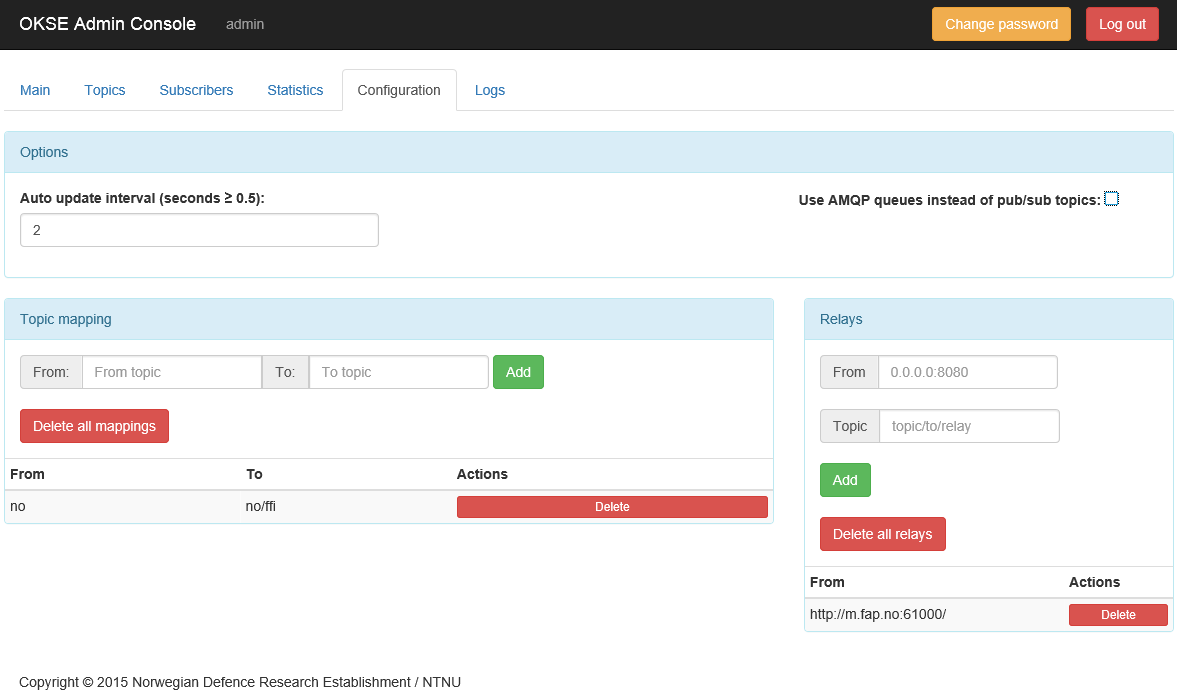
\includegraphics[width=\textwidth]{fig/oac/configurationpane.png}}
    \caption{The OKSE Admin Console - Configurations pane} 
    \label{fig:OKSE Admin Console - Configurations pane}
  \end{figure}
\end{center}

\subsection{The Logs pane}
The main feature of the "Logs" pane is the large text area, providing all of the information printed from the application. Logging is separated into 4 levels, "ERROR", "WARN", "INFO" and "DEBUG". The "DEBUG" level shows the full set of messages printed during system runtime. "INFO" prints messages that are meant to show the progress and events happening in the application. The "WARN" level prints messages that might potentially lead to system failure. Finally, "ERROR" shows events which has caused a failure in the system. There are one button for each of the message types, allowing the user to filter out information. The "Lines" area, lets the user decide how many lines of information that are displayed. Lastly, the "Stop refresh" buttons stops new messages from showing up in the text-area.

\begin{center}
  \begin{figure}[ht!]
    \makebox[\textwidth]{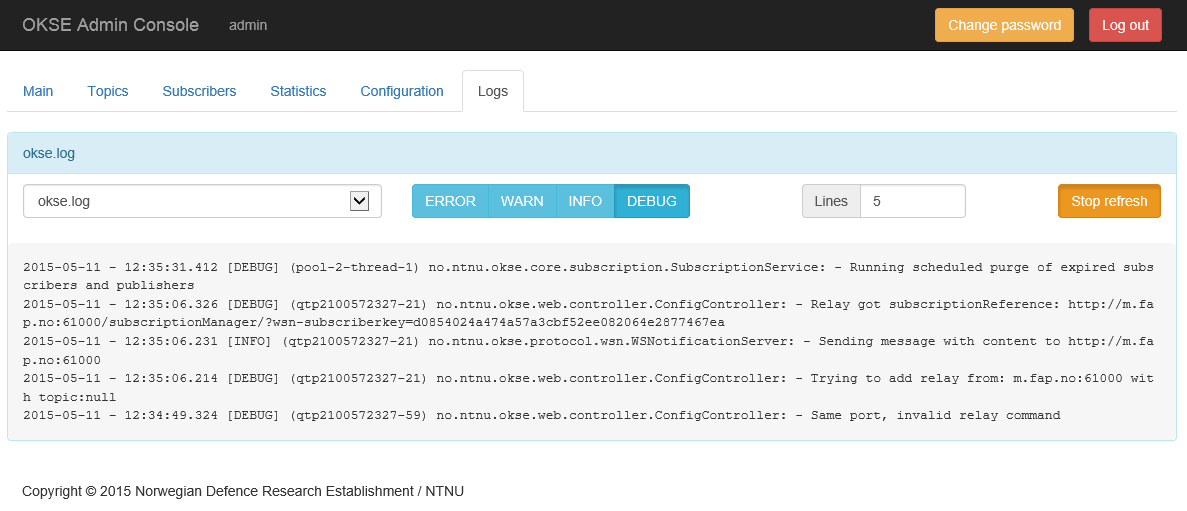
\includegraphics[width=\textwidth]{fig/oac/logpane.png}}
    \caption{The OKSE Admin Console - Logs pane} 
    \label{fig:OKSE Admin Console - Logs pane}
  \end{figure}
\end{center}

\section{Configuration files}
\label{sec:configuration_files}
OKSE has three configurations files. The main configuration file is the okse.properties file. You also got log4j.properties, and topicmapping.properties. This chapter describe the default configuration.

\subsection{okse.properties}
\label{subsec:configuration_files-okse.properties}
 
 This is the main configuration file within the system. See below for a detailed list of all possible settings, and their description.

\begin{description}
\setlength{\itemsep}{0cm}%
  \item[sprint.application.name] \hfill \\
  Application name to be displayed in the Admin Console \hfill \\ Default: \verb!OKSE Message Broker!
  \item[server.port] \hfill \\
  Tells Jetty which port the Admin Console should use \hfill \\ Default: \verb!8080!
  \item[ADMIN\_PANEL\_HOST] \hfill \\
  The host the Admin Console should use \hfill \\ Default: \verb!0.0.0.0!
  \item[CACHE\_MESSAGES] \hfill \\
  Tells OKSE if it should cache messages \hfill \\ Default: \verb!true!
  \item[BROADCAST\_SYSTEM\_MESSAGES\_TO\_SUBSCRIBERS] \hfill \\
  Tells OKSE if system messages shoudl be broadcasted to all subscribers \hfill \\ Default: \verb!false!
  \item[ENABLE\_WSNU\_DEBUG\_OUTPUT] \hfill \\
  Tells OKSE if it should log WSNU \hfill \\ Default: \verb!false!
  \item[DEFAULT\_SUBSCRIPTION\_TERMINATION\_TIME] \hfill \\
  Tells OKSE what the subscription termination time should be \hfill \\ Default: \verb!15552000000!
  \item[DEFAULT\_PUBLISHER\_TERMINATION\_TIME] \hfill \\
  Tells OKSE what the publisher termination time should be \hfill \\ Default: \verb!15552000000!
  \item[TOPIC\_MAPPING] \hfill \\
  Tells OKSE the path to the topic mapping configuration file \hfill \\ Default: \verb!config/topicmapping.properties!
  \item[WSN\_HOST] \hfill \\
  Tells OKSE what host WSNotificanServer should listen to \hfill \\ Default: \verb!0.0.0.0!
  \item[WSN\_PORT] \hfill \\
  Tells OKSE what port WSNotificationServer should listen to \hfill \\ Default: \verb!61000!
  \item[WSN\_CONNECTION\_TIMEOUT] \hfill \\
  Tells OKSE what connection timeout to use with WS-Notification \hfill \\ Default: \verb!5!
  \item[WSN\_POOL\_SIZE] \hfill \\
   WSNotification http client thread pool used to queue outbound requests \hfill \\ Default: \verb!50!
   \item[WSN\_MESSAGE\_CONTENT\_ELEMENT\_NAME] \hfill \\
  Tells OKSE what name non-XML content should be wrapped in \hfill \\ Default: \verb!Content!
  \item[WSN\_USES\_NAT] \hfill \\
  Tells OKSE if it's hosted behind NAT/Port forwarded network \hfill \\ Default: \verb!false!
  \item[WSN\_WAN\_HOST] \hfill \\
  Tells OKSE what host it's behind when using NAT \hfill \\ Default: \verb!test.doman.com!
  \item[WSN\_WAN\_PORT] \hfill \\
  Tells OKSE what port it's behind when using NAT \hfill \\ Default: \verb!61000!
  \item[DUMMYPROTOCOL\_HOST] \hfill \\
  Tells OKSE what host DummyProtocolServer should listen to \hfill \\ Default: \verb!0.0.0.0!
  \item[DUMMYPROTOCOL\_PORT] \hfill \\
  Tells OKSE what port DummyProtocolServer should listen to \hfill \\ Default: \verb!61001!
  \item[AMQP\_HOST] \hfill \\
  Tells OKSE what host AMQPProtocolServer should listen to \hfill \\ Default: \verb!0.0.0.0!
  \item[AMQP\_PORT] \hfill \\
  Tells OKSE what port AMQPProtocolServer should listen to \hfill \\ Default: \verb!5672!
  \item[AMQP\_USE\_QUEUE] \hfill \\
  Tells OKSE if AMQP should use the standard queue or the non-standard topic implementation \hfill \\ Default: \verb!false!
  \item[AMQP\_USE\_SASL] \hfill \\
  Tells OKSE if AMQP should use SASL \hfill \\ Default: \verb!true!
  \item[spring.resources.cache-period] \hfill \\
  Tells Spring what cache-period to set on HTTP-requests \hfill \\ Default: \verb!1!
  \item[spring.thymeleaf.suffix] \hfill \\
  Tells Spring what all Thymeleaf templates are suffixed with \hfill \\ Default: \verb!.html! 
   \item[spring.thymeleaf.mode] \hfill \\
  Tells Spring what type all Thymeleaf templates are \hfill \\ Default: \verb!HTML5!
   \item[spring.thymeleaf.encoding] \hfill \\
  Tells Spring what encoding to use on all Thymeleaf templates \hfill \\ Default: \verb!UTF-8!
   \item[spring.thymeleaf.content-type] \hfill \\
  Tells Spring what content-type all Thymeleaf templates should be returned with \hfill \\ Default: \verb!text/html! 
\end{description}
  
 \subsection{log4j.properties}
 \label{subsec:log4j.properties}
 
This is the configuration file for all the log files available for the system. See below for a detailed list of all possible settings, and their description.

\begin{description}

\setlength{\itemsep}{0cm}%
  \item[log] \hfill \\
  Default folder location for log files, relative to .jar file \hfill \\ Default: \verb!logs!
  \item[pattern] \hfill \\
  Default pattern to print log output in \hfill \\ Default: \verb!%d{yyyy-MM-dd - HH:mm:ss.SSS} [%p] (%t) %c: - %m%n!
   \item[maxLogFileSize] \hfill \\
  Max log file size, before log rotate \hfill \\ Default: \verb!5MB!
   \item[numberOfBackups] \hfill \\
  Max number of log files, before it purges old files \hfill \\ Default: \verb!10!
   \item[log4j.logger.no.ntnu.okse] \hfill \\
  Default log level for okse log messages \hfill \\ Default: \verb!DEBUG, OKSE!
  \item[log4j.logger.org.apache.qpid] \hfill \\
  Default log level for qpid log messages \hfill \\ Default: \verb!DEBUG, QPID!
  \item[log4j.logger.org.eclipse.jetty] \hfill \\
  Default log level for Jetty log messages \hfill \\ Default: \verb!INFO, JETTY!
  \item[log4j.logger.org.springframework] \hfill \\
  Default log level for Spring log messages \hfill \\ Default: \verb!INFO, SPRING!
  
  \item[log4j.appender.OKSE] \hfill \\
  Default appender to use for OKSE logs \hfill \\ Default: \verb!org.apache.log4j.RollingFileAppender!
  \item[log4j.appender.OKSE.File] \hfill \\
  Default log file to use for OKSE logs \hfill \\ Default: \verb!${log}/okse.log!
   \item[log4j.appender.OKSE.MaxFileSize] \hfill \\
  Default log file size to use for OKSE logs \hfill \\ Default: \verb!${maxLogFileSize}!
   \item[log4j.appender.OKSE.MaxBackupIndex] \hfill \\
  Number of backups for OKSE logs \hfill \\ Default: \verb!${numberOfBackups}!
   \item[log4j.appender.OKSE.layout] \hfill \\
  Pattern engine for OKSE logs \hfill \\ Default: \verb!org.apache.log4j.PatternLayout!
   \item[log4j.appender.OKSE.layout.conversionPattern] \hfill \\
  Default pattern to use for OKSE logs \hfill \\ Default: \verb!${Pattern}!

    \item[log4j.appender.SPRING] \hfill \\
  Default appender to use for SPRING logs \hfill \\ Default: \verb!org.apache.log4j.RollingFileAppender!
  \item[log4j.appender.SPRING.File] \hfill \\
  Default log file to use for SPRING logs \hfill \\ Default: \verb!${log}/spring.log!
   \item[log4j.appender.SPRING.MaxFileSize] \hfill \\
  Default log file size to use for SPRING logs \hfill \\ Default: \verb!${maxLogFileSize}!
   \item[log4j.appender.SPRING.MaxBackupIndex] \hfill \\
  Number of backups for SPRING logs \hfill \\ Default: \verb!${numberOfBackups}!
   \item[log4j.appender.SPRING.layout] \hfill \\
  Pattern engine for SPRING logs \hfill \\ Default: \verb!org.apache.log4j.PatternLayout!
   \item[log4j.appender.SPRING.layout.conversionPattern] \hfill \\
  Default pattern to use for SPRING logs \hfill \\ Default: \verb!${Pattern}!

  \item[log4j.appender.JETTY] \hfill \\
  Default appender to use for JETTY logs \hfill \\ Default: \verb!org.apache.log4j.RollingFileAppender!
  \item[log4j.appender.JETTY.File] \hfill \\
  Default log file to use for JETTY logs \hfill \\ Default: \verb!${log}/okse.log!
   \item[log4j.appender.JETTY.MaxFileSize] \hfill \\
  Default log file size to use for JETTY logs \hfill \\ Default: \verb!${maxLogFileSize}!
   \item[log4j.appender.JETTY.MaxBackupIndex] \hfill \\
  Number of backups for JETTY logs \hfill \\ Default: \verb!${numberOfBackups}!
   \item[log4j.appender.JETTY.layout] \hfill \\
  Pattern engine for JETTY logs \hfill \\ Default: \verb!org.apache.log4j.PatternLayout!
   \item[log4j.appender.JETTY.layout.conversionPattern] \hfill \\
  Default pattern to use for JETTY logs \hfill \\ Default: \verb!${Pattern}!
  
    \item[log4j.appender.QPID] \hfill \\
  Default appender to use for QPID logs \hfill \\ Default: \verb!org.apache.log4j.RollingFileAppender!
  \item[log4j.appender.QPID.File] \hfill \\
  Default log file to use for QPID logs \hfill \\ Default: \verb!${log}/qpid.log!
   \item[log4j.appender.QPID.MaxFileSize] \hfill \\
  Default log file size to use for QPID logs \hfill \\ Default: \verb!${maxLogFileSize}!
   \item[log4j.appender.QPID.MaxBackupIndex] \hfill \\
  Number of backups for QPID logs \hfill \\ Default: \verb!${numberOfBackups}!
   \item[log4j.appender.QPID.layout] \hfill \\
  Pattern engine for QPID logs \hfill \\ Default: \verb!org.apache.log4j.PatternLayout!
   \item[log4j.appender.QPID.layout.conversionPattern] \hfill \\
  Default pattern to use for QPID logs \hfill \\ Default: \verb!${Pattern}!

 \item[log4j.appender.stdout] \hfill \\
  Default appender to use for console output \hfill \\ Default: \verb!org.apache.log4j.ConsoleAppender!
   \item[log4j.appender.stdout.Target] \hfill \\
  Default target to use for console output \hfill \\ Default: \verb!System.out!
    \item[log4j.appender.stdout.layout] \hfill \\
  Pattern engine for console logs \hfill \\ Default: \verb!org.apache.log4j.PatternLayout!
   \item[log4j.appender.stdout.layout.conversionPattern] \hfill \\
  Default pattern to use for console logs \hfill \\ Default: \verb!${Pattern}!
  
 \end{description}
 
 \subsection{topicmapping.properties}
 \label{subsec:topicmapping.properties}
 
 This is a configuration file for adding predefined topic mappings to be available when the broker boots. The mapping is asyncron. This means that the broker forward messages from one topic to another one, but not back again (TopicA forward to TopicB, but not visa versa). If you want syncron forwarding (A to B, and B to A), you have to add two mappings, A=B and B=A. By default, there are no topic mapping listed. To add predefined topic mappings, use the following format: \verb!from=to!. An example mapping is: \verb!no/ffi=nato/hq/info!.
This will forward all messages received on no/ffi to nato/hq/info
 
\section{Test clients}
As none of the protocols has any useful clients for testing, we have provided a JAR file for AMQP send  and one for AMQP receive. Keep in mind that the time spent on these clients are very small, and that they are only suitable for minor testing. As the groups task was not to implement clients, they do only run from command line with the arguments given below.

\subsection{AMQP send}
Provided in the project delivery there is a folder named misc-jars, within this folder, the file amqpsend.jar is located. The file takes three arguments.

\begin{description}
    \item[-a amqp://localhost:5672/topic] \hfill \\
  Address argument, needed to tell what server to send the message to \hfill \\ Default: \verb!amqp://localhost:5672/example!
    \item[-s "subject"] \hfill \\
  Subject argument, not needed. \hfill \\ Default: \verb!example!
    \item[message] \hfill \\
  The last argument will be sent as the message \hfill \\ Default: \verb!example!
\end{description}
Below an example of a valid command is shown, the message in the example is sent to the localhost:
\verb!java -jar amqpsend.jar -a amqp://localhost/test -s "test" test!

\subsection{AMQP receive}
Provided in the project delivery there is a folder named misc-jars, within this folder, the file amqprecv.jar is located. The file takes one argument.
 
\begin{description}
    \item[-a amqp://localhost:5672/topic] \hfill \\
  Address argument, tells the receiver where to subscribe \hfill \\ Default: \verb!amqp://localhost:5672/example!
\end{description}
Below an example of a valid command is shown, the receiver will subscribe to localhost:
\verb!java -jar amqprecv.jar -a amqp://localhost/test!

\subsection{WSN Test script}
Under the development of the application, there was a need for a test script to generate valid WSN messages to test different aspects of the validator. The script can be used to send different kind of messages over WSN, but \textit{cannot} receive messages.

The script is written in Python 2.7 and uses a third party plugin called requests\footnote{\url{http://docs.python-requests.org/en/latest/}}. This script should run on any platform as long as Python and requests is available. Below, an installation guide for Windows, Linux and OS X.

\subsubsection{Windows}
To install Python and requests on a Windows machine, you will need to go through the following steps:

\begin{enumerate}
\setlength{\itemsep}{0cm}%
    \item Download and install the latest version of Python 2.7 from python.org
    \item Open cmd.exe
    \item Change directory to python27 by entering: cd C:/Python27
    \item Install requests by running the command: python -m pip install requests
\end{enumerate}

After the installation, change directory of the cmd session to the location of bullrider.py. To run python in the shell in any directory, the Python2.7 directory should be added to the path. This can be done for the current session by entering the command: \verb!path %path%;C:\Python27!.
Note that this will have to be done for every new cmd.exe window you open.

Now that Python and requests is installed, move on to the Usage section (\ref{}).

\subsubsection{Linux/OS X}
Mac OS X and most Linux distributions comes with Python 2.7 installed. To verify that you have Python 2.7 installed, open a terminal and write "python". You should see something like:
\begin{verbatim}
$ python
Python 2.7.9 (default, Mar  1 2015, 12:57:24)
[GCC 4.9.2] on linux2
\end{verbatim}

If you get command not found, consult your package manager on how to install Python 2.7 or go to python.org and download the installer from there.

When Python 2.7 is installed, we need to install requests. In the terminal, the command pip, or easy\_install will be available. If the pip command is available, install requests using the following command:

\begin{verbatim}
    pip install requests
\end{verbatim}

If pip is not available use easy\_install in the following way:

\begin{verbatim}
    easy_install requests
\end{verbatim}

After the installation, change directory in the terminal to the location of bullrider.py.

Now that Python and requests is installed, move on to the Usage section (\ref{}).


\subsubsection{Usage}
To use the bullrider.py script, you need a terminal/cmd.exe window that is changed to the directory of bullrider.py. If you are using Windows, remember to repeat the path step if Python is not permanently added to your path. 

Bellow is a description on what the different arguments do, and the available options that can be used. Note that the arguments need to be given in the listed order.

The format of the arguments is as follows:

\verb!python bullrider.py [request type] [hostname/ip] [port] [topic]!


\begin{description}
    \item[request type] \hfill \\
  Type of request to send, available: all, notify, massnotify, multinotify, subscribe, unsubscribe \hfill \\ Default: \verb!None!
    \item[hostname/ip] \hfill \\
  Hostname or IP address of the OKSE instance \hfill \\ Default: \verb!None!
    \item[port] \hfill \\
  Port of the OKSE instance \hfill \\ Default: \verb!None!
    \item[topic] \hfill \\
  The topic to send the given request to. \hfill \\ Default: \verb!None!
\end{description}
Below an example of a valid command is shown, this will send a notify to a OKSE hosted on localhost at port 61000:

\verb!python bullrider.py notify localhost 61000 example!

\section{Troubleshooting}

If you encounter any problems with the software, check the following points before you contact the development team: 

\begin{itemize}
\setlength{\itemsep}{0cm}%
\item Do you have the correct JRE? For OKSE Message Broker to run properly, you need version 8 or newer. Other versions than this may cause problems, or not work at all.
\item Network connectivity. Verify that your network connection is working and that the ports are open. Also ensure that you use port forwarding if you don't have a public IP. 
\end{itemize}

\clearpage